\documentclass[tikz,border=8pt]{standalone}
\usepackage{amsmath,amssymb}
\usetikzlibrary{arrows.meta,calc,decorations.markings,decorations.pathmorphing,patterns,shapes.geometric,positioning}

\begin{document}
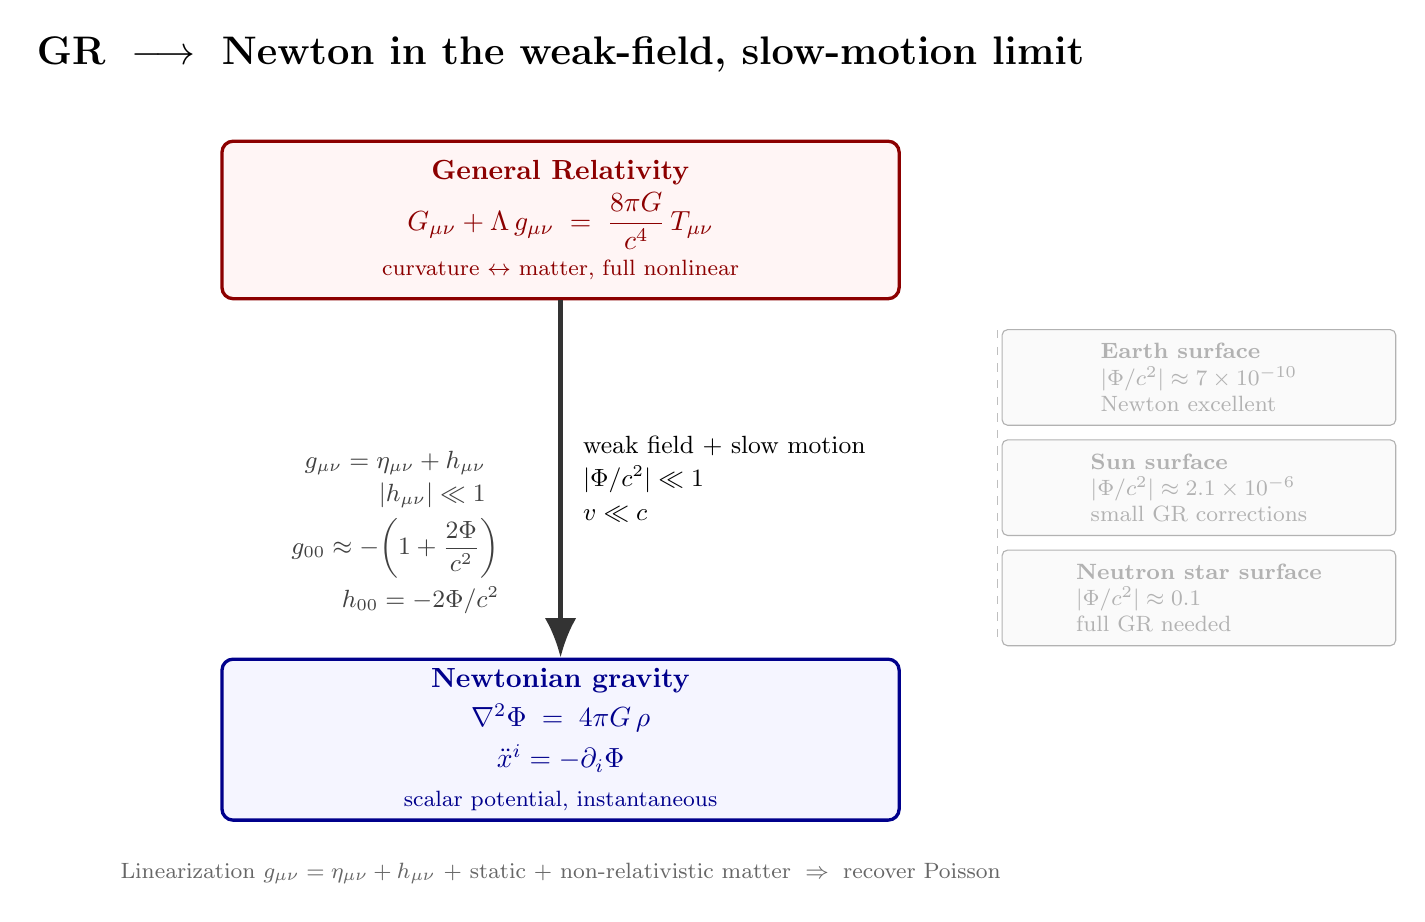
\begin{tikzpicture}[>=Latex,
    grbox/.style={draw, very thick, red!55!black, fill=red!4, rounded corners=4pt,
                  minimum width=8.6cm, minimum height=2.0cm, align=center, font=\normalsize},
    nbox/.style={draw, very thick, blue!55!black, fill=blue!4, rounded corners=4pt,
                  minimum width=8.6cm, minimum height=2.0cm, align=center, font=\normalsize},
    bigarrow/.style={-{Latex[length=5mm,width=4mm]}, line width=1.6pt, black!80},
    sidebox/.style={draw, thin, gray!60, fill=gray!4, rounded corners=2pt,
                  minimum width=5.0cm, align=left, font=\footnotesize, inner sep=5pt}]

  % --- TOP: GR ---
  \node[grbox] (gr) at (0, 4.0)
    {\textbf{General Relativity}\\[2pt]
     $G_{\mu\nu} + \Lambda\, g_{\mu\nu} \;=\; \dfrac{8\pi G}{c^{4}}\, T_{\mu\nu}$\\[3pt]
     \footnotesize curvature $\leftrightarrow$ matter, full nonlinear};

  % --- BOTTOM: Newton ---
  \node[nbox] (nw) at (0, -2.6)
    {\textbf{Newtonian gravity}\\[2pt]
     $\nabla^{2}\Phi \;=\; 4\pi G\,\rho$\\[3pt]
     $\ddot{x}^{i} = -\partial_{i}\Phi$\\[2pt]
     \footnotesize scalar potential, instantaneous};

  % --- ARROW from GR -> Newton ---
  \draw[bigarrow] (gr.south) -- (nw.north)
    node[midway, right=4pt, font=\small, align=left, text=black]
    {weak field + slow motion\\[1pt]
     $|\Phi/c^{2}| \ll 1$\\[1pt]
     $v \ll c$};

  % Mid-label on the LEFT of arrow
  \node[font=\small, align=right, text=black!75] at (-2.1, 0.7)
    {$g_{\mu\nu} = \eta_{\mu\nu} + h_{\mu\nu}$\\[1pt]
     $|h_{\mu\nu}| \ll 1$};

  \node[font=\small, align=right, text=black!75] at (-2.1, -0.4)
    {$g_{00} \approx -\!\left(1 + \dfrac{2\Phi}{c^{2}}\right)$\\[2pt]
     $h_{00} = -2\Phi/c^{2}$};

  % --- RIGHT-SIDE: weak-field ladder ---
  \node[sidebox, anchor=west] (earth) at (5.6, 2.0)
    {\textbf{Earth surface}\\
     $|\Phi/c^{2}| \approx 7\times 10^{-10}$\\
     Newton excellent};

  \node[sidebox, anchor=west] (sun)   at (5.6, 0.6)
    {\textbf{Sun surface}\\
     $|\Phi/c^{2}| \approx 2.1\times 10^{-6}$\\
     small GR corrections};

  \node[sidebox, anchor=west] (ns)    at (5.6, -0.8)
    {\textbf{Neutron star surface}\\
     $|\Phi/c^{2}| \approx 0.1$\\
     full GR needed};

  % small connecting decoration: vertical line linking the three boxes
  \draw[thin, dashed, gray!50] (5.55, 2.6) -- (5.55, -1.4);

  % Title strip on top
  \node[font=\Large\bfseries, align=center] at (0, 6.1)
    {GR $\;\longrightarrow\;$ Newton in the weak-field, slow-motion limit};

  % Bottom note
  \node[font=\footnotesize, align=center, text=black!60] at (0, -4.3)
    {Linearization $g_{\mu\nu}=\eta_{\mu\nu}+h_{\mu\nu}$ + static + non-relativistic matter
     $\;\Rightarrow\;$ recover Poisson};

\end{tikzpicture}
\end{document}
